% ---------------------------------------------------------------------------
% Workshop paper, Section 4 (Experiments). Condensed from thesis Chapter 5.
% Kept : offline tables 5.1/5.2/5.3 restricted to the released baseline,
%        RoboRef-Std and RoboRef-Asym; MetaWorld (fig 5.7); Robomimic.
% Cut  : all Qwen3.5 rows, all RoboRef-ICL rows, the "with demonstration"
%        columns (meaningless without the ICL exposition), LIBERO entirely,
%        the LoRA recipe study, and the deployment-configuration table
%        (compressed into prose under "Protocol").
% ---------------------------------------------------------------------------
\section{Experiments}
\label{sec:results}

We compare three reward models: the released \textbf{Robometer-4B} baseline,
\textbf{RoboRef-Std}, our fine-tune on the re-curated corpus with Robometer's
original symmetric losses, and \textbf{RoboRef-Asym}, the same fine-tune with the
asymmetric objective of Section~\ref{sec:method-loss}. RoboRef-Std is the control
that separates our two contributions: it sees exactly our failure data and
differs from RoboRef-Asym in the objective alone.

\subsection{Offline reward quality}
\label{sec:results-offline}

We evaluate on two splits: one held out from our own corpus, and Robometer's
held-out-embodiment set, which is out of distribution for every model.

\begin{table}[t]
\centering\footnotesize
\caption{Offline ranking, in distribution, by the progress head. Rank accuracy is
the fraction of success--failure pairs ordered correctly; $\tau$ is Kendall's
correlation with true frame order. Higher is better.}
\label{tab:offline-id-rank}
\begin{tabular}{@{}lcc@{}}
\toprule
Model & rank-acc & $\tau$ \\
\midrule
Robometer-4B (released) & $0.611$ & $0.437$ \\
RoboRef-Std             & $0.771$ & $0.591$ \\
RoboRef-Asym            & $\mathbf{0.846}$ & $\mathbf{0.692}$ \\
\bottomrule
\end{tabular}
\end{table}

\begin{table}[t]
\centering\footnotesize
\caption{Offline success detection, in distribution. The success head is the
signal downstream RL reads, so its precision--recall area, its true-positive rate
at a five-percent false-positive budget, and its ROC area matter most; $d'$ is
the class separation of the progress head. Higher is better.}
\label{tab:offline-id-succ}
\begin{tabular}{@{}lcccc@{}}
\toprule
Model & AUPRC & TPR@5\%FPR & ROC-AUC & $d'$ \\
\midrule
Robometer-4B (released) & $0.67$ & $0.24$ & $0.67$ & $0.42$ \\
RoboRef-Std             & $0.88$ & $0.51$ & $0.87$ & $1.08$ \\
RoboRef-Asym            & $\mathbf{0.89}$ & $\mathbf{0.54}$ & $\mathbf{0.88}$ & $\mathbf{1.31}$ \\
\bottomrule
\end{tabular}
\end{table}

\begin{table}[t]
\centering\footnotesize
\setlength{\tabcolsep}{4pt}
\caption{Offline evaluation out of distribution, on a $571$-episode
held-out-robot set spanning six robots no model saw in training. The progress
head is decoded as the mean conditioned on the model having moved off its lowest
bin, since the fine-tuned heads are bimodal on this set; this leaves the
baseline, whose distributions are unimodal, unchanged. Higher is better.}
\label{tab:offline-ood}
\begin{tabular}{@{}lcccc@{}}
\toprule
 & \multicolumn{2}{c}{success head} & \multicolumn{2}{c}{progress head} \\
\cmidrule(lr){2-3}\cmidrule(lr){4-5}
Model & AUC & TPR@5\% & rank-acc & $\tau$ \\
\midrule
Robometer-4B (released) & $\mathbf{0.86}$ & $\mathbf{0.38}$ & $\mathbf{0.81}$ & $\mathbf{0.63}$ \\
RoboRef-Std             & $0.76$ & $0.16$ & $0.76$ & $0.50$ \\
RoboRef-Asym            & $0.79$ & $0.28$ & $\mathbf{0.81}$ & $0.58$ \\
\bottomrule
\end{tabular}
\end{table}

In distribution our fine-tunes win across the board. At the strict five-percent
false-positive budget, the operating point that matters for a reward a policy
will optimize against, they recover $0.51$--$0.54$ of true successes against the
baseline's $0.24$ (Table~\ref{tab:offline-id-succ}). RoboRef-Std, which changes
nothing of Robometer's recipe but the training data, already carries most of that
gain: rank accuracy rises from $0.611$ to $0.771$ and the TPR more than doubles.
The asymmetric loss adds a further, smaller margin on every column, most visibly
on class separation, $d' = 1.08 \to 1.31$.

Out of distribution the picture is different and worth stating plainly: the
released baseline leads three of the four columns
(Table~\ref{tab:offline-ood}). Our fine-tunes remain competitive on the progress
head, where RoboRef-Asym matches the baseline's rank accuracy, but neither
recovers its success-head calibration on embodiments none of the models has seen.
Offline, then, the honest summary is that we are clearly stronger in
distribution and no better out of it.

\subsection{Downstream reinforcement learning}
\label{sec:results-rl}

\paragraph{Protocol.}
Offline evaluation scores a reward on trajectories it is handed. The deployment
test reverses that, letting an optimizing policy query the reward on its own
rollouts. We train image-based IBRL policies and score each by \emph{true} task
success, measured in a separate evaluation where the reward model is never
queried, so the curves report ground truth and not the reward the policy reads.
Our models read the success head alone, as a sparse reward that terminates the
episode the moment the success probability crosses a threshold. Every reward
model, ours and the published baselines, is calibrated by one shared procedure on
a small set of held-out oracle rollouts, so calibration cannot be what separates
them; and every model is given a per-task minimum episode length, below which a
success signal is ignored, which suppresses an early-training exploit where a
policy provokes a spurious success before the task is physically solvable. The
published baselines, RoboReward, RoboDopamine and LRM, each run in the
configuration their authors intend, with their richest inputs and native reward
forms, which favours them; our comparison is therefore conservative.

\begin{figure*}[t]
\centering
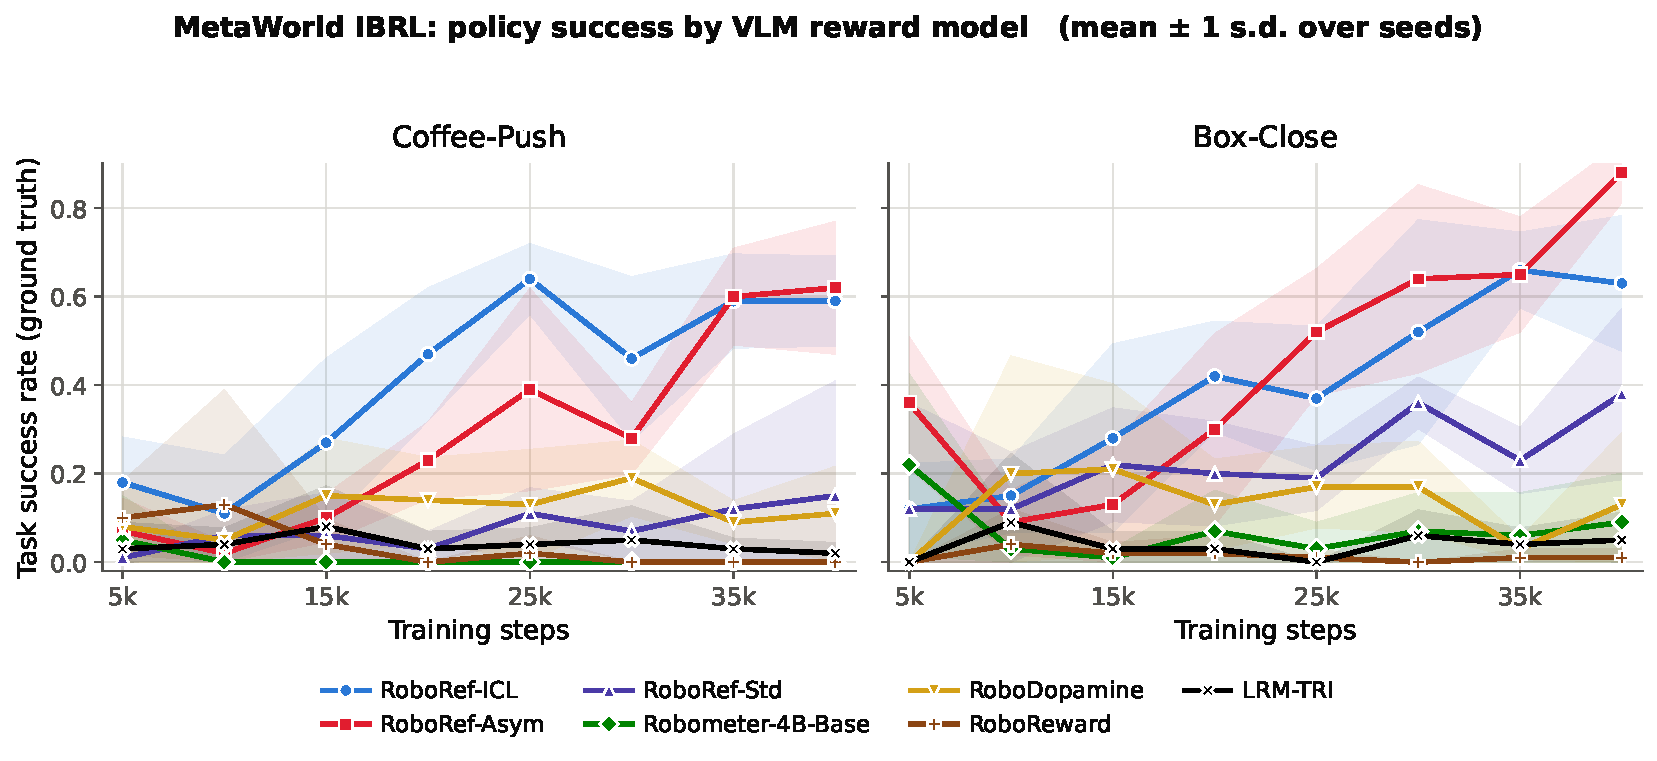
\includegraphics[width=\textwidth]{media/results/metaworld_rl.pdf}
\caption{MetaWorld downstream RL on two held-out tasks absent from every reward
model's training data, five seeds per reward, mean ground-truth success with a
one standard deviation band. Only the asymmetric fine-tune trains a competent
policy; every other reward ends far behind.}
\label{fig:mw-rl}
\end{figure*}

\paragraph{MetaWorld: the success head, and the offline--online gap.}
Figure~\ref{fig:mw-rl} is the widest separation we measure. RoboRef-Asym reaches
a mean success of $0.50$ on Coffee-Push and $0.72$ on Box-Close. Nothing else
comes close: the three published baselines stay under $0.13$ throughout, and the
released Robometer-4B, strong enough offline to reproduce its own paper's
numbers, moves the policy almost nowhere, $0.00$ and $0.07$ under its better
form.

The informative curve is RoboRef-Std. Offline it looked the part, recovering half
of all successes at the strict budget (Table~\ref{tab:offline-id-succ}). Under an
optimizing policy it comes apart, $0.11$ and $0.32$, well short of the asymmetric
fine-tune trained on the same trajectories. The entire distance between them is
the loss. What read offline as a modest edge in class separation, $d'$ of $1.08$
against $1.31$, is on-policy the line between a reward a policy exploits and one
it cannot. This is the paper's central observation: a fixed test set measures how
often a reward is right on average, while an optimizing policy hunts for the
specific states where it is wrong. The asymmetric loss does not make the reward
more accurate on average; it makes it \emph{hard to exploit}, and that, not
offline accuracy, is what decides whether a policy can be trained.

\begin{figure*}[t]
\centering
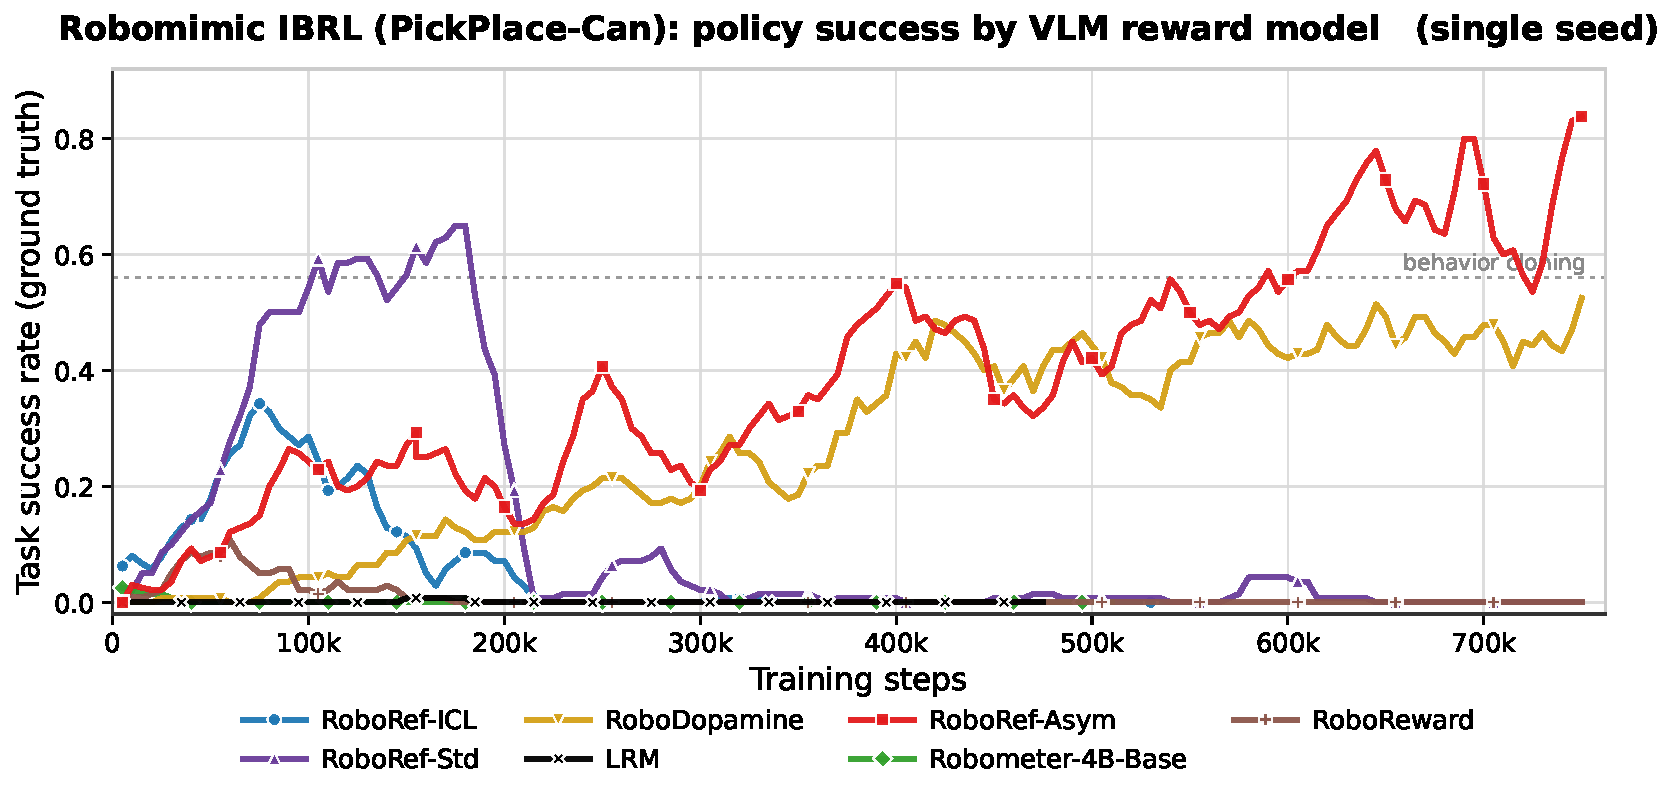
\includegraphics[width=0.72\textwidth]{media/results/robomimic_rl.pdf}
\caption{Robomimic PickPlace-Can, a domain absent from every reward model's
training data, one seed per reward, smoothed ground-truth success over $750$k
steps. The dashed line marks the behavior-cloning policy IBRL starts from, at
$0.56$. RoboRef-Asym is the only reward that ends above it.}
\label{fig:robomimic-rl}
\end{figure*}

\paragraph{Robomimic: out of distribution.}
No reward model here ever trained on Robomimic's scenes or rendering. Because
IBRL starts from a behavior-cloning policy, the dashed line at $0.56$ in
Figure~\ref{fig:robomimic-rl} is the bar that matters: a curve ending above it
has learned something the demonstrations alone could not teach. One reward clears
it. RoboRef-Asym climbs for essentially the whole run, passes the cloning line
near $590$k steps, and is still rising at $0.84$ when the budget ends. Among the
baselines only RoboDopamine trains a real policy, reaching $0.53$, recovering the
competence already in the demonstrations without moving beyond it.

RoboRef-Std is the fastest starter, above the cloning line within roughly $105$k
steps and peaking at $0.65$, then falling to zero in the space of a few
evaluations and never returning. Its only differences from the released baseline,
flat at zero for the entire run, are our training data and the dropped preference
head. The failure supervision alone turns a reward that never moves a policy on
this domain into one that drives genuine learning, and the asymmetric loss is
what lets the model keep that gain rather than lose it to the false positives a
symmetric objective leaves standing.

% =========================================================================
% TODO(maniskill): NO RESULTS YET. The 5-seed x {RoboRef-Asym, baseline}
% PullCube-v1 sweep at 300k steps is queued but has not run, and the earlier
% numbers were never logged and are not recoverable. Do NOT fill this in
% from memory. Once the runs land, this paragraph needs: final eval success
% per model (mean over 5 seeds), and the figure below.
%
% \begin{figure*}[t]
% \centering
% \includegraphics[width=\textwidth]{media/results/maniskill_rl.pdf}
% \caption{ManiSkill PullCube-v1 downstream RL, five seeds per reward, mean
% ground-truth success over $300$k steps, with the progress head supplying a
% dense per-step reward and no termination.}
% \label{fig:maniskill-rl}
% \end{figure*}
%
% \paragraph{ManiSkill: the progress head.}
% Both benchmarks above read the success head. ManiSkill tests the other head,
% the one the re-curated failure data most directly targets: dense per-step
% progress, supplying the entire reward, with no VLM termination and no
% ground-truth leak through \texttt{done}.
% =========================================================================
